\begin{figure}[t]
\centering
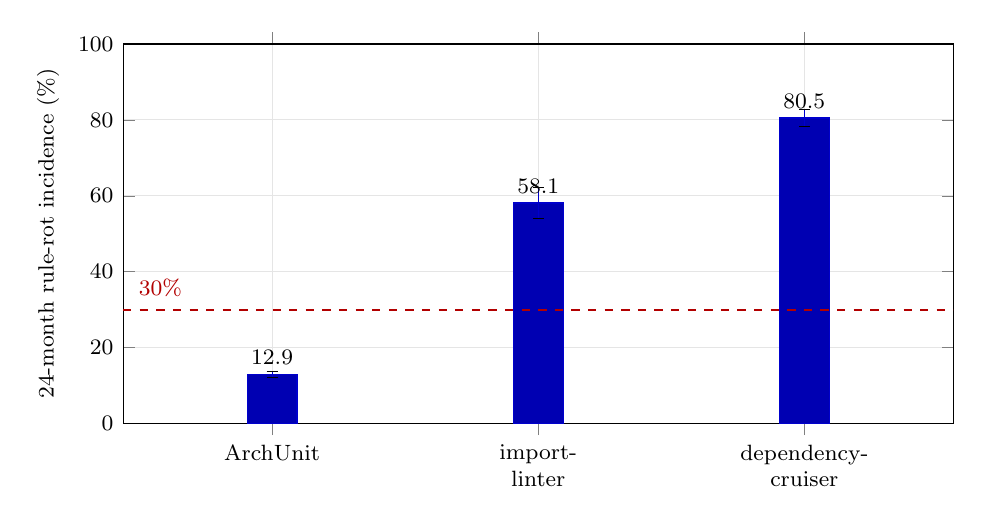
\begin{tikzpicture}
\begin{axis}[
  ybar,
  width=\columnwidth,
  height=6.4cm,
  ymin=0, ymax=100,
  ylabel={24-month rule-rot incidence (\%)},
  symbolic x coords={ArchUnit,import-linter,dependency-cruiser},
  xtick=data,
  xticklabels={ArchUnit,{import-\\linter},{dependency-\\cruiser}},
  xticklabel style={font=\footnotesize, align=center},
  nodes near coords,
  every node near coord/.append style={font=\footnotesize},
  bar width=18pt,
  enlarge x limits=0.28,
  tick label style={font=\footnotesize},
  label style={font=\footnotesize},
  grid=major,
  major grid style={gray!20},
  error bars/y dir=both,
  error bars/y explicit,
]
\addplot[fill=blue!70!black, draw=blue!80!black, error bars/.cd, y dir=both, y explicit]
  coordinates {
    (ArchUnit,12.9) +- (0,0.85)
    (import-linter,58.1) +- (0,4.15)
    (dependency-cruiser,80.5) +- (0,2.15)
  };
\draw[dashed, red!70!black, thick]
  (current axis.west |- {axis cs:ArchUnit,30}) --
  (current axis.east |- {axis cs:ArchUnit,30})
  node[above, font=\footnotesize, red!70!black, pos=0, anchor=south west, xshift=2pt, yshift=1pt] {$30\%$};
\end{axis}
\end{tikzpicture}
\caption{Kaplan-Meier survival analysis of rule rot by tool.}
\label{fig:survival_analysis}
\end{figure}
